%!TEX program=luatex

\newpage
\pagenumbering{arabic}
\section{Introduction}
La première motivation de ce travail est de fournir un outil qui enchaîne les processus de catégorisation et de recommandation des articles de presse, et pour chaque article un processus de résumé automatique et un autre de traduction automatique. Pour parvenir a réaliser cet ensemble de processus en deux langues (Anglais et Arabe), nous proposons une architecture de base de notre programme "Akhbirni" pour la réalisation de cet outil. 

\section{Présentation de l’architecture modulaire du système Akhbirni}

L’architecture du système "Akhbirni" se décline en quatre processus (catégorisation des articles, Recommandation, Résumé automatique des articles, Traduction automatique des articles). Les entrées (articles de presse extraits de plusieurs sources) sont sauvegardés dans une base de données. Le processus de catégorisation commence par classer les articles selon leur sujet, le processus de recommandation prend le relais ensuite pour recommander de façon personnalisé les articles. Enfin dés que les données sont prêtes, le résumé automatique et la traduction automatique seront mis en place pour chaque article comme le montre la figure ci-dessous (figure x).

\begin{figure}[H]
    \centering
    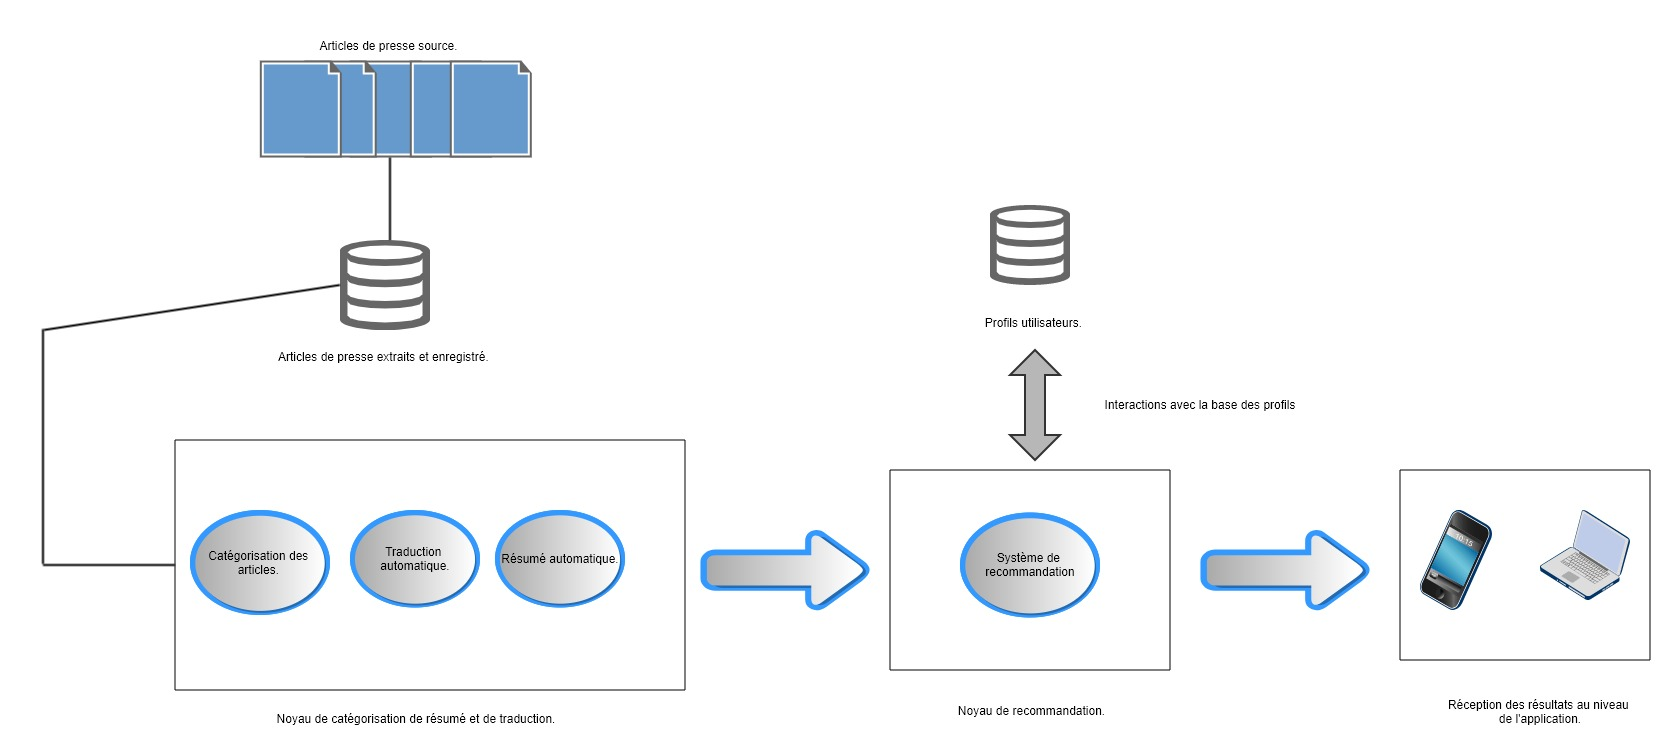
\includegraphics[height=300pt,width=500pt]{img/chapter3/globsche.jpg}
    \caption{Architecture globale du système.}
\end{figure}


\subsection{Architecture du module stockage des articles}
Le module de stockage des articles de notre système est composé des données sur les articles de presse extraits depuis les plateformes sources, a cet effet nous avons choisi \emph{JSON} qui est un format léger d'échange de données. Il est facile à lire ou à écrire pour des humains\cite{json} et est pris en charge par tout les langages de programmation. Les articles sont représentés comme suit :

   \begin{itemize}
    
     \item Un identifiant "Id": pour chaque article un identifiant unique lui est attribué.\\
     
     \item Un titre "Titre" : on sauvegarde le titre de chaque article.\\
     
     \item Un auteur "Auteur" : on sauvegarde le nom de l'auteur.\\
     
     \item Un description "Description" : on stocke la description de l'article originale (en cas de disponibilité).\\
     
     \item Le lien de l'article "LienArticle" : On stocke le lien de l'article originale.\\
     
     \item Le lien de l'image de l'image de l'article "LienImage" : On stocke le lien de l'image de l'article originale.\\
     
     \item Une date de publication "DatePublication" : On sauvegarde la date de publication de l'article originale.\\
     
    \end{itemize}

     \begin{lstlisting}[style=code]
      #Exemple de la structure d'un fichier JSON pour un article
      articles": [
     -{
     "Id":"124001",
     "Titre": "Alibaba Expects Revenue to Jump in the Next Year",
     "Auteur": "Liza Lin",
     "Description": "Alibaba says it expects revenue to grow 60% in the next year, as its core commerce business and cloud computing business attracts more customers.",
     "LienArticle": "https://www.wsj.com/articles/alibabas-profit-falls-as-e-commerce-giant-ramps-up-investments-1525435046",
     "LienImage": "https://images.wsj.net/im-9384/social",
     "DatePublication": "2018-05-04T14:21:00Z",
     },
     
     \end{lstlisting}
    
\subsection{Architecture du module stockage des profils}
Le module de stockage des profils de notre système est lui assez similaire a celui des articles, il regroupe des informations sur les utilisateurs, en plus des informations standards (Nom,Prénom,Adresse), on retrouve entre autre le vecteur de préférences. Ces informations son représentés comme suit :

\begin{itemize}
    
    \item Un identifiant "Id": pour chaque utilisateur un identifiant unique lui est attribué.\\
    
    \item Un Nom "Nom" : on sauvegarde le Nom de chaque utilisateur.\\
    
    \item Un Prénom "Prénom" : on sauvegarde le prénom de chaque utilisateur.\\
    
    \item Une adresse "Adresse" : on sauvegarde l'adresse de chaque utilisateur (pour une éventuelle localisation).\\
    
    \item Une liste de préférences "Préférences" : On stocke les préférences des utilisateurs sous-forme d'un vecteur clé-valeur.\\
    
\end{itemize}

\begin{lstlisting}[style=code]
#Exemple de la structure d'un fichier JSON pour un utilisateur
articles": [
-{
"Id":"22",
"Nom": "Kheloufi",
"Prénom": "Yanis",
"Adresse": "Alger, Algerie",
"Préférences": {
          "Technology": "0.63",
          "Business": "0.42",
          },
},
\end{lstlisting}


\subsection{Architecture du module de recommandation}
Les entrées de ce module sont des articles de presses de notre bases de données des articles décrite précédemment, trois types de recommandations sont faites :\\

\subsubsection{Filtrage basé similarité}
Dans ce processus, la tache principale est de recommander une liste d'articles potentiellement similaires par l'évaluation de la similarité de cosinus entre l'article qui est lu et les articles présent dans la base de données.
 
\subsubsection{Filtrage collaboratif (collaborative filtering)}
Comme il a été défini dans le premier chapitre, le filtrage collaboratif fait la recommandation des articles préférés des utilisateurs selon la similarité entre les utilisateurs. L'évaluation de la similarité de cosinus entre les préférences de plusieurs utilisateurs (deux ou plus) permet de recommander a un utilisateur un article susceptible de le plaire. 
Nous allons donc, regrouper les utilisateurs ayant des intérêts similaires par le calcul de similarité le plus adéquat.

\subsection{Architecture du module de résumé automatique}
Dans ce module, nous avons implémenté une technique de résumé automatique basé sur l'extraction des phrases les plus importantes en utilisant les plongement de mots (word embedding) selon \cite{extractiveword2vec}. Ci-dessous une description détaillé des procédures de résumé automatique :

\begin{figure}[H]
    \centering
    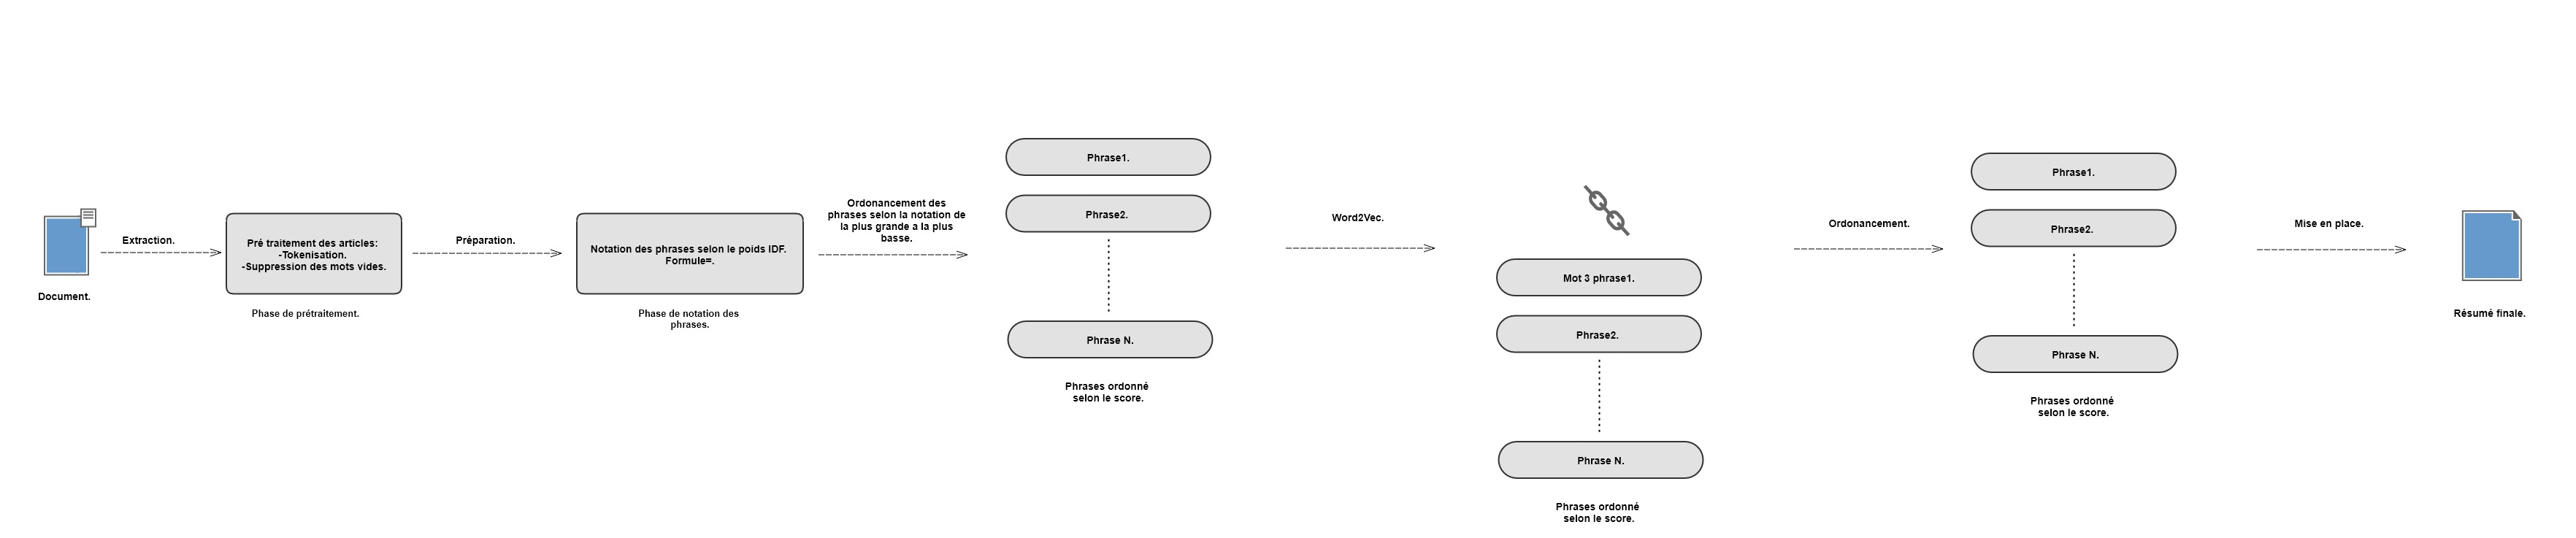
\includegraphics[height=150pt,width=500pt]{img/chapter3/ressche.jpg}
    \caption{Architecture globale du système.}
\end{figure}


\subsection{Architecture du module de catégorisation}
Dans ce module, la catégorisation se fait a l'arrivé d'un nouveau flux d'articles suivant les étapes suivantes :

\begin{figure}[H]
    \centering
    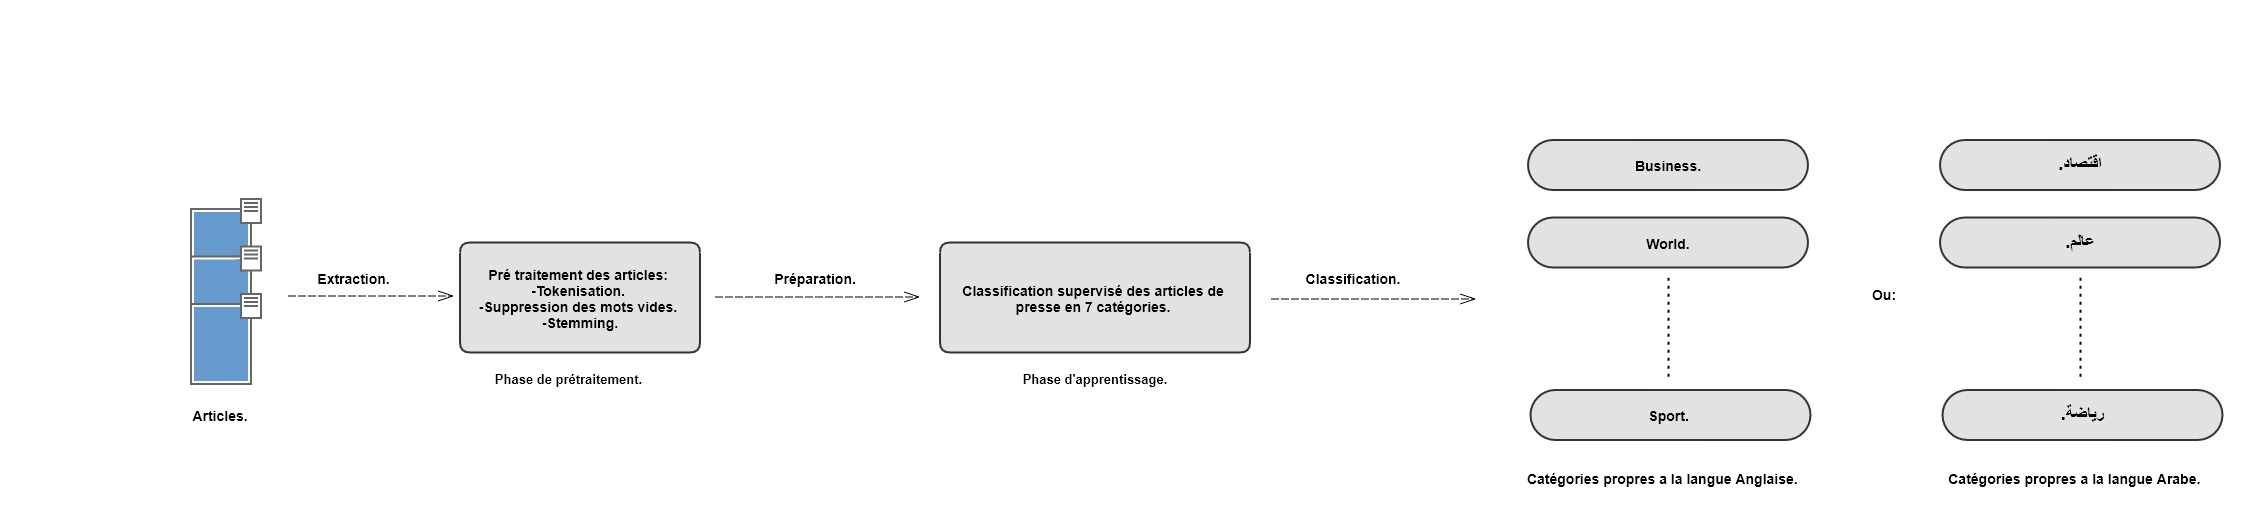
\includegraphics[height=150pt,width=500pt]{img/chapter3/categsche.jpg}
    \caption{Architecture globale du système.}
\end{figure}

\begin{itemize}
    
    \item \textbf{Prétraitement des articles:}
    A l'arrivée d'un nouveau article le module de catégorisation exécute un prétraitment qui englobe entre autre les étapes de Tokenisation, suppression des mots vides,stemming et mises en place des n-grammes.
    A la fin de cette étape, l'article est prêt a être classifié.\\
    
    \item \textbf{La classification:}
    La classification est la tache la plus importante de ce module, a cet effet, nous avons décidé de mettre en place un modèle basé sur un apprentissage automatique supervisé \emph{SVM} compte tenu des résultats démontrés dans les articles \cite{}\cite{}.\\ 

\end{itemize}



\subsection{Architecture du module de traduction automatique}
Dans ce module, notre tache n'était pas d'implémenter ou de concevoir un traducteur automatique, mais uniquement d'utiliser un traducteur automatique multilingue déjà existant et de l'intégrer dans notre architecture globale présenté dans la (figure1.1). Toutefois, il fallait rechercher le module de traduction le plus performant afin de traduire un article complet de la manière la plus rapide.

\subsection{Architecture du serveur}


\section{Présentation de l’architecture fonctionnelle de Akhbirni}

\subsection{Fonctionnement du système}

Lors de l'introduction de l'utilisateur dans le système "akhbirni", une demande d'authentification est alors affichée, la suite de la navigation peut être alors :

\subsubsection{personnalisé}

si l'utilisateur s'authentifie, la version personnalisé de notre système lui sera accessible et pourra :

Dès la 1ère connexion de cet utilisateur, il sera amené à Choisir ses catégories favorites afin d'établir son profil utilisateur, ensuite il aura accès aux articles classé et suggérés selon ses choix (catégories). Pour chaque article, l'utilisateur pourra bénéficier de :
 
\begin{itemize}
    
    \item \textbf{Recommandation personnalisé:}
    Sur la base d'articles sélectionnés précédemment, le module de recommandation va établir une liste d'articles susceptibles d'intéresser l'utilisateur de l'application.
    
    \item \textbf{Consultations des articles recommandé:}
    Après avoir établi une liste d'articles recommandés, le système retournera cette liste au niveau de l'interface graphique et permettra ainsi a l'utilisateur de bénéficier des articles recommandés.
        
    \item \textbf{Catégorisation automatique des articles:}
    Les articles sont catégorisés afin de représenter au mieux notre bases des articles.
    
    \item \textbf{Résumé automatique:}
    Au lieu de lire un article complet, l'utilisateur aura un résumé généré automatiquement a partir de l'article qui lui permettra de retrouver tout les faits importants décrit dans l'article.
    
    \item \textbf{Traduction automatique:}
    l'utilisateur aura la possibilité de faire une traduction de l'article en cours de lecture si il le désire et cela en différentes langues.

    \item \textbf{Enregistrer des articles:}
    l'utilisateur aura la possibilité d'enregistrer l'article en cours de lecture si il le désire, et le retrouver sur l'application.
    
    \item \textbf{Ajouter des mentions de préférences:}
    l'utilisateur aura la possibilité d'ajouter une mention de préférence "j'aime" ou "je n'aime pas" sur l'article.

    \item \textbf{Recherche des articles:}
    l'utilisateur aura la possibilité de faire une recherche spécifique des articles, et ceux en se basant soit sur : une recherche basé mots clés, une recherche basé sur une catégorie ou une recherche selon la source de l'article. 
    
\end{itemize}

Dès la connexion de l’utilisateur, ce dernier peut s’identifier en utilisant un nom d’utilisateur et un mot de passe ; sinon il utilisera les services non personnalisés du système.

\subsubsection{non personnalisé}
Dans l'autre cas, si l'utilisateur ne souhaite pas adhérer a l'application, la version non personnalisé sera entièrement accessible et il pourra :

\begin{itemize}
    
    \item \textbf{Recommandation basé similarité:}
    Dans le cas non personnalisé, la recommandation se basera uniquement sur l'article recherchés et lu par l'utilisateur, puisque le système va calculer la similarité entre l'article lu et ceux dans la base de données des articles pour retourner une liste d'articles similaires.
    
    \item \textbf{Consultation des articles suggérés:}
    l'utilisateur pourra en effet au moment même ou il lit un article, d'avoir une suggestion d'autres articles jugés similaires par le système.
    
    \item \textbf{Catégorisation automatique des articles:}
    Les articles sont catégorisés afin de représenter au mieux notre bases des articles.
    
    \item \textbf{Résumé automatique:}
    l'utilisateur reçoit avec l'article, un résumé automatique de ce dernier.
    
    \item \textbf{Traduction automatique:}
    l'utilisateur aura la possibilité de faire une traduction de l'article en cours de lecture si il le désire et cela en différentes langues.
    
    \item \textbf{Recherche des articles:}
     l'utilisateur aura la possibilité de faire une recherche spécifique des articles, et ceux en se basant soit sur : une recherche basé mots clés, une recherche basé sur une catégorie ou une recherche selon la source de l'article. 
    
    
\end{itemize}

\section{Schémas conceptuels du système akhbirni}

La conception de notre système désigne la façon dont le logiciel fournit les différentes fonctionnalités recherchées. Ainsi, nous allons présenter les fonctionnalités de notre application et les acteurs influent sur le fonctionnement de celle-ci. Afin d'expliciter la conception de notre système, nous avons choisi la méthode UML (Unified Modeling Language), qui est une notation graphique conçue pour représenter, spécifier et construire les systèmes logiciels. UML utilise des techniques orientées objets pour la modélisation des systèmes, depuis la conception jusqu'à la maintenance, d’une manière compréhensible par l’homme et disposant de qualités formelles suffisantes pour être traduites automatiquement en code source.\cite{uml}

\subsection{Diagramme de cas d'utilisation}
"Le diagrammes de cas d'utilisation (initié par Ivar Jacobson en 1992 dans la méthode OOSE) est un type de diagramme UML qui permet de définir les besoins des acteurs dans un système quelconque en établissant les fonctionnalités attendues et en organisant les besoins. Il peut être aussi utilisés ensuite comme moyen d’organisation du développement du logiciel, notamment pour la structuration et le déroulement des tests du logiciel".\cite{uml}\\

Ces principaux composants sont :

\begin{itemize}
    
    \item \textbf{Acteur:}
    
    Un acteur est un utilisateur type qui a toujours le même comportement vis-à-vis d’un cas d’utilisation. Les utilisateurs d'un système appartiennent a une ou plusieurs classes d’acteurs selon les rôles qu’ils tiennent par rapport au système. Il est a noter que, une même personne physique peut se comporter en autant d’acteurs différents que le nombre de rôles qu’elle joue vis-à-vis du système et que un acteur peut aussi être un système externe avec lequel le cas d’utilisation va interagir.\cite{uml}
    
    \begin{figure}[H]
        \centering
        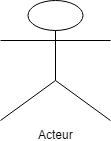
\includegraphics[height=90pt,width=90pt]{img/chapter3/ActeurUML.png}
        \caption{Modélisation d'un acteur.}
    \end{figure}
    
    
    \item \textbf{Cas d'utilisation:}
    Un cas d’utilisation correspond à un certain nombre d’actions que le système devra exécuter en réponse à un besoin d’un acteur. Un cas d’utilisation doit produire un résultat observable pour les acteurs du système.
    
\begin{figure}[H]
    \centering
    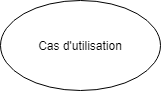
\includegraphics[height=90pt,width=90pt]{img/chapter3/CasutilisationUML.png}
    \caption{Modélisation d'un Cas d'utilisation.}
\end{figure}


    \item \textbf{Relations entre cas d'utilisation:}

    \item \textbf{Relations entre acteurs:}
    
    
\end{itemize}

\subsubsection{Diagramme de cas d'utilisation de Akhbirni}

    \begin{figure}[H]
    \centering
    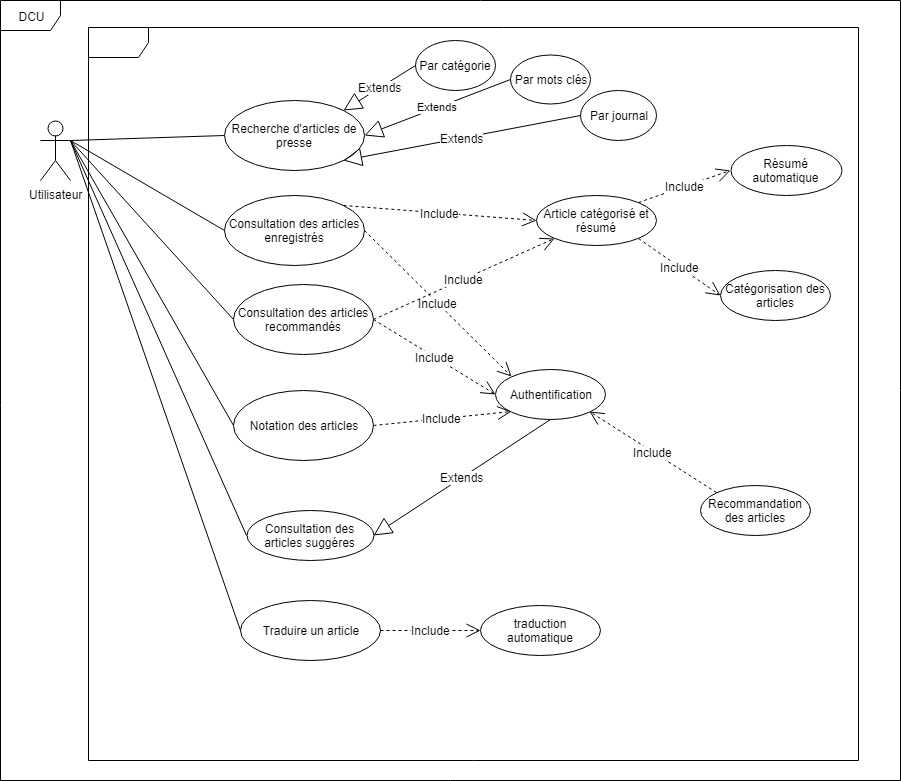
\includegraphics[height=300pt,width=300pt]{img/chapter3/Cas_d'utilisation.jpg}
    \caption{Modélisation d'un Cas d'utilisation.}
    \end{figure}

\subsection{Diagramme de classe}
Le diagramme de classe est l'un des pivots essentiels de la modélisation avec UML car il décrit la structure statique d'un système. En effet, aucun détail ni traitement sont représenté dans ce diagramme puisque il 
se base uniquement sur la notion d'objet, de classe (comprenant des attributs et des opérations) et les différents types d'associations entre les classes.\\

Ces principaux composants sont :

\begin{itemize}
    
    %%[Hamilton et Russell, 2006, Charroux et al. 2009, Pilone et Pitman, 2005]
    
    \item \textbf{Classe :} 
    Une classe décrit un groupe d’objets ayant les mêmes propriétés (attributs), un même comportement (opérations), et une sémantique commune (domaine de définition).\\
    
    \item \textbf{Objet :} Un objet est l’instance d’une classe. Pour notre cas, prenons « Ouvrier », c’est une
    instance de la classe « Employé ».
    
    \begin{itemize}
        
    \item Attributs : Un attribut est une propriété élémentaire d’une classe. Pour chaque objet d’une classe, l’attribut prend une valeur (sauf cas d’attributs multivalués).
    
    \item Méthodes : Une méthode est l’implémentation d’une opération. Chaque classe par défaut inclut plusieurs méthodes, qui décrivent ses opérations.
    
    
   \end{itemize}
    
    \item \textbf{Relations:}
    En UML, il existe plusieurs façons pour décrire les relations entre les classes. Chaque relation exprime un dépendance particulière qui peut être de différents types :
    
    \begin{itemize}
        
    \item Association : L'association est le premier niveau de relation entre 2 classes. Elle spécifie tout simplement qu'une classe peut en utiliser une autre. Graphiquement, elle est sous la forme d’un trait plein, jointe à un label décrivant la relation souvent avec un verbe à l’infinitif. Donc dans une Société, Poste est associé à un Employé.
    
    
    \item Agrégation : C’est une relation plus forte qu’une association. Contrairement à l’association,l’agrégation représente une relation d’inclusion structurelle ou comportementale d’un ensemble. De plus, l’agrégation est une relation transitive. En se basant toujours sur le même exemple, une Société a plusieurs Employés.
    
    
    \item Composition : Appelée aussi « agrégation composite », elle représente une agrégation particulière. Sa particularité est qu’elle est l’auteur de la création et la destruction d’objets. Dans le cas d’une société, les départements sont les composites de la société. Donc si la société se dissout alors les départements seront aussi défaits.
    
    \item Héritage : C’est un principe abstrait. Il donne la possibilité de diviser récursivement les objets en plusieurs ensembles (parties), où chaque partie est une classe. Revenons à notre exemple, un ingénieur, un ouvrier, un agent de sécurité, appartiennent tous à la classe « Employé ». Pour un besoin conceptuel, où on aura besoin de les séparer pour leur ajouter des attributs spécifiques à chaque grade d’employés. Donc les valeurs de l’attribut « Grade » de la classe Employé sont reprise sous forme de classes qui héritent de la classe mère « Employé ». Par conséquent, toutes
    les classe enfants vont hériter toutes les caractéristiques (Attributs, Méthodes, Relations) de la classe mère

   \end{itemize}

\end{itemize}

\subsubsection{Diagramme de classe de Akhbirni}

\begin{figure}[H]
    \centering
    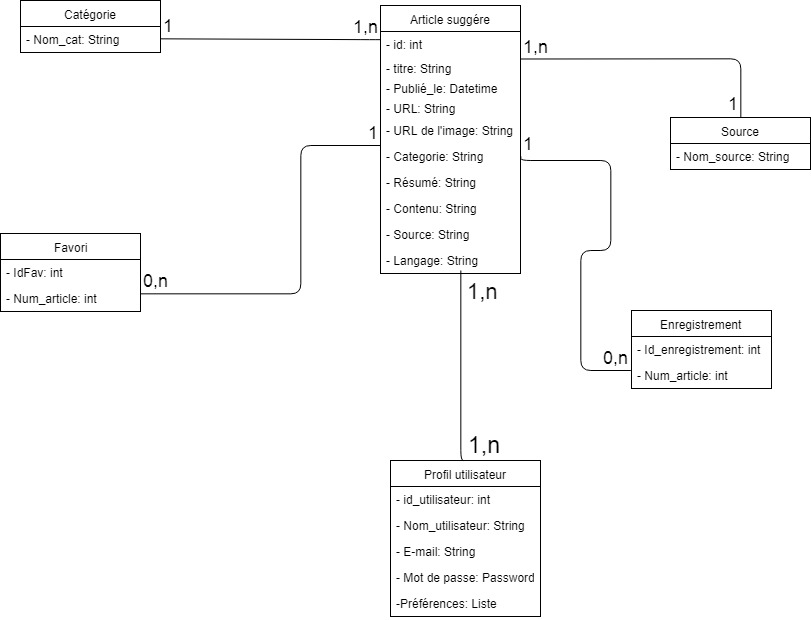
\includegraphics[height=500pt,width=400pt]{img/chapter3/ClassDiagram.jpg}
    \caption{Diagramme de classe akhbirni}
\end{figure}

\subsection{Diagramme de séquence}
Le diagramme de séquence est un diagramme UML qui fait partie des diagrammes comportementaux (dynamiques) dont L’objectif est de représenter les interactions entre les objets et les acteurs ou bien entre objets uniquement  en indiquant la chronologie des échanges. Cette représentation peut se réaliser en considérant les différents scénarios associés.

Un diagramme de séquence est composé d’un
ensemble d’objets, où chaque objet a une ligne de vie, ainsi qu’un ensemble de messages.Ces principaux composants sont :

\begin{itemize}
  
    \item \textbf{Les Objets :}
    Le diagramme de séquence est composé de plusieurs objets qui interagissent entre eux à l’aide de messages. Un objet est représenté par un rectangle avec le nom de l’objet à l’intérieur.
    
    \item \textbf{Ligne de vie :}
    Chacun des objets a sa propre ligne de vie, qui peut être considérée comme un axe temporel, elle est représentée par une ligne discontinue. Cette ligne de vie indique la période de vie de l’objet et elle se termine par une croix qui indique la destruction de l’objet.
        
       exemple :
       
       \begin{figure}[H]
        \centering
        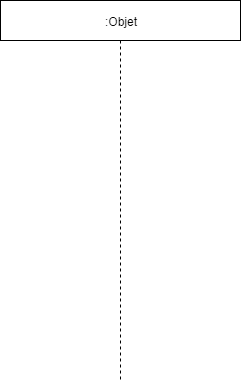
\includegraphics[height=150pt,width=150pt]{img/chapter3/objet_ligne.png}
        \caption{Modélisation d'un objet et d'une ligne de vie}
       \end{figure}
       
        
    \item \textbf{Les messages :}
     Un message représente une information envoyée de la part d’un objet A à un autre objet B. Il y’a deux types de messages, qui sont les suivants :
    
    \begin{itemize}
        
    \item Messages synchrones : La réception d’un message synchrone provoque un lancement obligatoire d’une de ces méthodes. D’où l’expéditeur reste bloqué jusqu'à la fin de l’exécution de cette méthode et réception d’une réponse. Les messages synchrones sont symbolisés par des flèches en pointillés.
    
    \item Messages asynchrones : Contrairement aux messages synchrones, l’envoi d’un message asynchrone ne bloque pas l’expéditeur de ce dernier. Ainsi l’expéditeur pourra continuer sa ligne de vie sans avoir à attendre une réponse. Les messages asynchrones sont symbolisés par des flèches pleines.
 
    \end{itemize}       

\end{itemize}

\subsubsection{Diagramme de séquence de Akhbirni}
\begin{figure}[H]
    \centering
    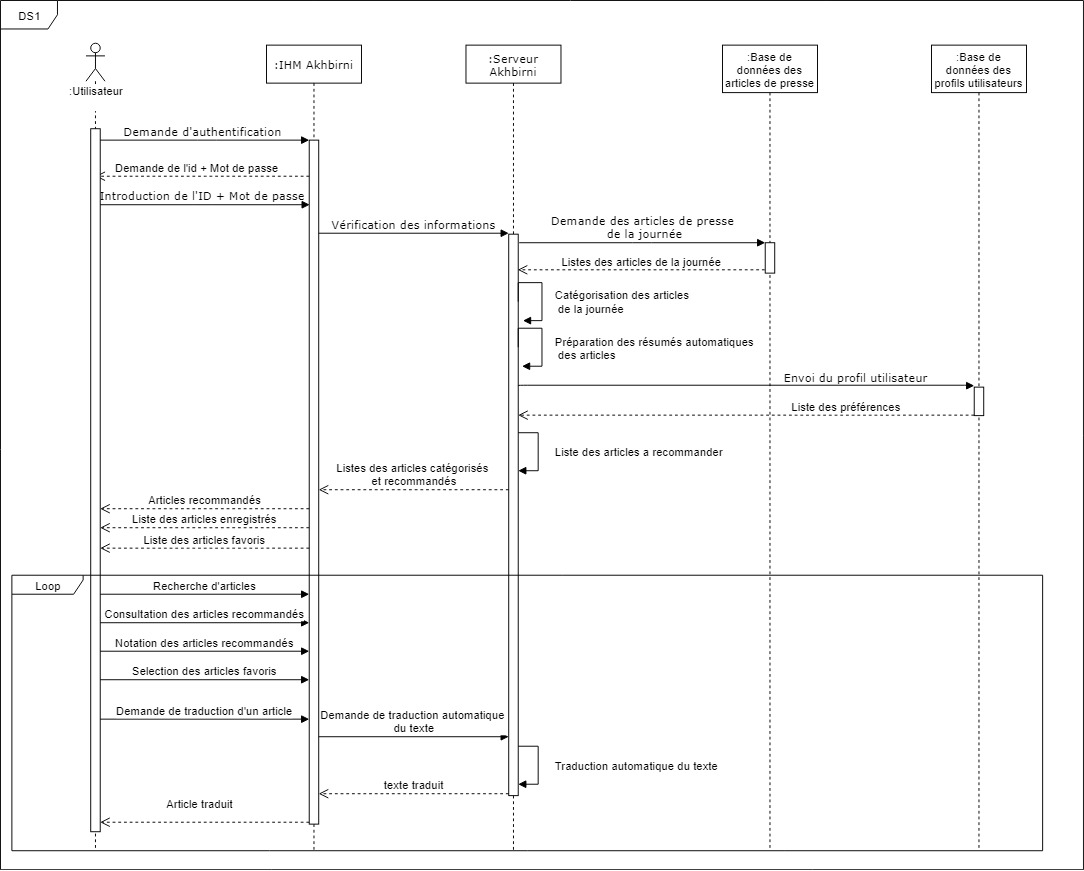
\includegraphics[height=500pt,width=450pt]{img/chapter3/diag_seq_pers.jpg}
    \caption{Diagramme de séquence dans le cas personnalisé}
\end{figure}


\begin{figure}[H]
    \centering
    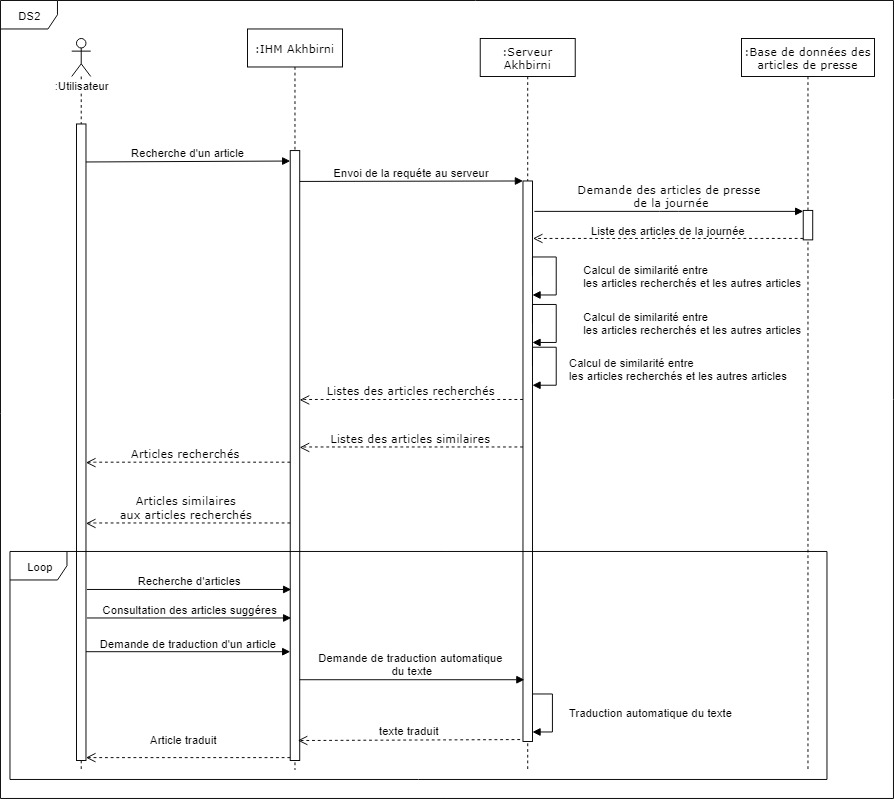
\includegraphics[height=500pt,width=450pt]{img/chapter3/diag_seq_nonpers.jpg}
    \caption{Diagramme de séquence dans le cas non personnalisé}
\end{figure}

\section{Conception du système}
Dans cette partie, nous étalerons plus de détails sur les modules conçue pour notre système.
On retrouve:

\subsection{Conception des bases de données}

\subsubsection{Bases de données NoSql}

L'idée de NoSQL a été réintroduite en 2009 lors d'un événement sur la distribution bases de données. À ce moment-là, les principales raisons de passer aux bases de données NoSQL sont reprises: performance et la flexibilité. La performance est principalement axée sur le partage et la gestion des données, tandis que la flexibilité des données correspond aux données semi-structurées ou non structurées qui peut provenir du web. Déjà en 2011 les principales technologies non relationnelles étaient déjà connus et décrits en fonction de leur fonctionnement. Hecht et
Jablonski [11] a décrit les principales caractéristiques offertes par différents NoSQL des solutions telles que Voldemort, Redis, Riak, MongoDB, CouchDB, Cassandra, HBase, etc.

À partir de 2012 et jusqu'à aujourd'hui, les bases de données NoSQL ont été de plus en plus évalué et comparé aux SGBDR. Évaluation des performances exécutée par [16] comparé Cassandra, MongoDB et PostgreSQL. Il a été conclu que MongoDB est capable de fournir un haut débit, mais surtout quand il est utilisé comme un seul serveur.

MongoDB est une base de données orientée document écrite en C++ \cite{}[8]. Les objets sont stockés en série sous la forme BSON. le
les objets n'ont pas besoin d'avoir la même structure ou les mêmes champs et les champs communs n'ont pas besoin d'avoir le même type,
permettant ainsi un stockage de schéma flexible.A cet effet,nous avons choisi de concevoir une solution basé sur les bases de données NoSQL.

\subsubsection{Base de données des articles}

\begin{itemize}
    
    \item Un identifiant "Id": pour chaque article un identifiant unique lui est attribué.\\
    
    \item Un titre "Titre" : on sauvegarde le titre de chaque article.\\
    
    \item Un auteur "Auteur" : on sauvegarde le nom de l'auteur.\\
    
    \item Un description "Description" : on stocke la description de l'article originale (en cas de disponibilité).\\
    
    \item Le lien de l'article "LienArticle" : On stocke le lien de l'article originale.\\
    
    \item Le lien de l'image de l'image de l'article "LienImage" : On stocke le lien de l'image de l'article originale.\\
    
    \item Une date de publication "DatePublication" : On sauvegarde la date de publication de l'article originale.\\
    
    \item Un résumé
    
    \item Une Catégorie
    
    \item Une langue
    
    \item Une source
    
    
\end{itemize}

\begin{lstlisting}[style=code]
#Exemple de la structure d'un fichier JSON pour un article
articles": [
-{
"Id":"124001",
"Titre": "Alibaba Expects Revenue to Jump in the Next Year",
"Auteur": "Liza Lin",
"Description": "Alibaba says it expects revenue to grow 60% in the next year, as its core commerce business and cloud computing business attracts more customers.",
"LienArticle": "https://www.wsj.com/articles/alibabas-profit-falls-as-e-commerce-giant-ramps-up-investments-1525435046",
"LienImage": "https://images.wsj.net/im-9384/social",
"DatePublication": "2018-05-04T14:21:00Z",
"résumé",
"catégorie",
"langue",
"source",
},

\end{lstlisting}

\subsubsection{Base de données des utilisateurs}

\begin{itemize}
    
    \item Un identifiant "Id": pour chaque utilisateur un identifiant unique lui est attribué.\\
    
    \item Un Nom d'utilisateur "Nomutilisateur" : on sauvegarde le Nom de chaque utilisateur.\\
    
    \item Une adresse e-mail "E-mail" : on sauvegarde l'adresse e-mail de chaque utilisateur (pour une éventuelle confirmation).\\
    
    \item Une liste de préférences "Préférences" : On stocke les préférences des utilisateurs sous-forme d'un vecteur clé-valeur.\\
    
\end{itemize}

\begin{lstlisting}[style=code]
#Exemple de la structure d'un fichier JSON pour un utilisateur
articles": [
-{
"Id":"22",
"Nom": "Kheloufi.yanis",
"Email": "yan.khel@gmail.com",
"Préférences": {
"Technology": "0.63",
"Business": "0.42",
},
},
\end{lstlisting}

\subsection{Conception du module de recommandation}

\subsubsection{Recommandation non personnalisé}
La recommandation non personnalisé vise a recommander des articles pour des utilisateurs qui n'ont pas de profil (non authentifié), pour cela notre système effectue une recommandation selon le choix de lecture de l'utilisateur , c'est a dire par calcul de similarité entre l'article qui est entrain de lire et d'autres articles potentiellement similaires a celui-ci.\\

\subsubsection{Méthode de calcul de la similarité entre les articles}
Afin de satisfaire les utilisateurs désirant utilisé l'option non personnalisé du système, une liste de suggestions doit être émises a ces derniers. Pour cela, nous proposons une solution de recommandations basé uniquement sur l'article lu par l'utilisateur et qui est basé sur la similarité de cosinus.

En considérant P et Q comme des vecteurs, la similarité de cosinus entre une paire de vecteurs lignes p et q est calculée comme suit:

                                      \[cos(\pmb P, \pmb Q) = \frac {\pmb p \cdot \pmb q}{||\pmb p|| \cdot ||\pmb q||}\]


\subsubsection{Recommandation personnalisé}
La recommandation des articles aux utilisateurs se base sur les profils de ces derniers. En effet, le profilage utilisateur débute lorsque l'utilisateur s'authentifie pour la première fois et a chaque fois les informations relatives a ses préférences sont récoltés et traités.\\
Cette étape exige:

\subsubsection{Le profilage utilisateur}
Le profilage est la première partie de ce processus. Elle consiste à déterminer les centres d’intérêts d’un utilisateur tout en se basant sur les articles lues par ce dernier. Pour cela, nous avons décidé d’utiliser une méthode de calcul des préférences afin de mieux cibler les utilisateurs et pour garantir une solution conforme aux caractéristiques de la recommandation pour les articles de presse.

\subsubsection{Méthode de calcul des préférences}
Pour le calcul des préférences utilisateurs, nous avons décidé d'utiliser une méthode de calcul qui permet a la fois de résoudre les problèmes de récence et le démarrage a froid. Cette méthode testé s'avère très efficace par rapport aux méthodes existantes et décrites dans le premier chapitre puisqu'elle attribut une valeur numérique calculé pour chaque catégorie

elle est calculé comme suit : 

Si un article est sélectionné:
                                   \[p = (1-{\alpha}) {p} + {\alpha}\]

Sinon: 
                                     \[{p} = (1-{\alpha}) {p}\]

Où p est la probabilité de sélection et α est le degré de diminution du poids.

Dans notre cas:
                                   p=1/Nombre de catégories.
                                   α=0.1

au fur et a mesure la probabilité de sélection diminue si la catégorie n'est pas sélectionné, et la plus récente aura le un poids plus élevé. 

 \begin{algorithm}
    
    \begin{algorithmic}[1]
        \STATE Profilage
        \STATE Début
        \STATE \alpha \gets 0.1;
        \STATE p \gets 1/$Nombre_de_catégorie$;     
        \STATE dés l'authentification d'un utilisateur i charger ses préférences;
        \STATE préférences \gets préférences(i);    
        \STATE Si $Selection_Article$ Alors :;
        \STATE \[p(catégorie_article) \gets (1-{\alpha}) {p} + {\alpha}\];
        \STATE Pour toute catégorie != $catégorie_article$ Faire:
        \STATE \[p(catégorie) \gets (1-{\alpha}) {p} \] ;
        \STATE Fin Pour;
        \STATE Fin Si;  
        \STATE FIN
\end{algorithmic}
        
\end{algorithm}


\subsubsection{Méthode de calcul de la similarité entre utilisateurs}
Jusque la, la solution proposée traite le problème de personnalisation, mais afin de diversifier notre recommandation auprès de l'utilisateur, nous avons décidé de mettre en place une méthode de calcul de similarité qui va nous permettre de recommander des articles éventuellement intéressant par rapport a l'utilisateur. Selon \cite{collaborativeapachemahout} qui propose une étude détaillé sur les mesures de similarité pour le filtrage collaboratif, il en est sorti comme conclusion que la distance euclidienne était la mesure la plus adéquate vu sa précision élevée et son temps d'exécution bas par rapport aux autres mesures.\\
En considérant P et Q comme des vecteurs, la distance euclidienne entre une paire de vecteurs lignes p et q est calculée comme suit:

            \[d({p} ,{q})=d({q} ,{p})={\sqrt {(q_{1}-p_{1})^{2}+(q_{2}-p_{2})^{2}+\cdots +(q_{n}-p_{n})^{2}}}\\
            ={\sqrt {\sum _{i=1}^{n}(q_{i}-p_{i})^{2}}}\]
  
\begin{algorithm}
    
    \begin{algorithmic}[1]
        \STATE Diversité
        \STATE Début
        \STATE dés l'authentification d'un utilisateur i charger ses préférences;
        \STATE préférences = préférences(i);
        \STATE Pour chaque article dans la base des articles Faire:
        \STATE SI {$Distance_euclidienne(i,j) >= Seuil(j)$} Alors:
        \STATE préférences \gets préférences(j);
        \STATE Fin Si;  
        \STATE Fin Pour;
        \STATE Fin
    \end{algorithmic}
    
\end{algorithm}

\subsubsection{Algorithme de Recommandation}


\begin{algorithm}
    \begin{algorithmic}[1]
        \STATE Recommandation
        \STATE Début
        \STATE dés l'authentification d'un utilisateur i charger ses préférences ;\\
        \STATE Profilage(i) ;\\
        \STATE Diversité(i) ;\\
        \STATE Pour chaque article dans la base des articles Faire:
        $Liste_recommandations \gets article$;\\
        \STATE FinSI;
        \STATE FinPour;
        \STATE \quad Retourner $Liste_recommandations$;
        \STATE Fin
    \end{algorithmic}
\end{algorithm}


\subsection{Conception du module de Catégorisation des articles}
Pour ce module de catégorisation des articles de presse, nous avons conçues notre solution en se basant sur \cite{miusfbvimuab} présenté dans le chapitre précédent et qui utilise un modèle d'apprentissage automatique supervisé SVM. Aprés avoir construit une solution préalablement a l'aide de K-means ou LDA (Clustering), nous nous sommes aperçu que SVM donnait de bien meilleurs résultats.\\

\subsubsection{Prétraitement des articles}

\begin{itemize}
\item \textbf{Prétraitement des articles}
Dans cette phase , on a mis en place un tokeniser pour chaque langue et supprimer les mots vides. Par la suite, on a mis en place le stemming après plusieurs tests pour nous assurer de l'amélioration des résultats. Enfin, nous avons mis en place les n-grammes (unigramme, bigramme et trigramme).

\item \textbf{Extraction des termes:}
Les données de texte sont composées de termes regroupés en phrases et paragraphes. En utilisant le modèle d'espace vectoriel, on décompose les données textuelles en un ensemble de termes.\\
L'ensemble des termes contenu dans la collection de données et dont la valeur indique soit un présent (0 ou 1) ou valeur absente ou un poids pour le terme pour le point de données. Cette représentation est connue comme la représentation «Extraction de termes» et est le plus représentation couramment utilisée pour les modèles de données de texte.

\item \textbf{Affectation des poids:}
Dans le modèle d'espace vectoriel, les documents sont représentés en tant que vecteurs. La pondération à terme est un concept important qui détermine le succès ou l'échec de la classification. TF-IDF est une technique qui utilise TF et IDF pour déterminer le poids d'un terme. Le schéma TF-IDF est très populaire dans le domaine de la classification de texte et presque tous les autres schémas de pondération sont des variantes de ce schéma.
\end{itemize}


\subsubsection{Modèle de catégorisation}
En choisissant un modèle basé sur un apprentissage automatique supervisé, nous avons pris SVM comme référence pour classifier nos données.  

\subsubsection{Algorithme de catégorisation}

\begin{algorithm}
\begin{algorithmic}[1]

\STATE Algorithme
\STATE Début
\STATE Chargement du corpus d'apprentissage ;\\
\STATE Pr\'etraitement: Tokenisation, elimination des mots vides, stemming, Mise en place des ngrammes ;\\
\STATE Calcul de la fréquence des termes par document TF-IDF ;\\
\STATE Mise en place de l'apprentissage automatique supervisé avec SVM;\\
\STATE \quad Retourner Modèle;
\STATE Fin

\end{algorithmic}
\end{algorithm}


\subsection{Conception du module de résumé automatique}
Pour ce module de résumé automatique, nous avons choisi un résumeur automatique extractif de \cite{ffff} qui est basé sur les plongements de mots (Word embeddings) décrit dans le chapitre précédent.

\subsubsection{Prétraitement des articles}
Dans cette phase , il suffit juste de tokeniser le texte et supprimer les mots vides puisque le stemming ne peut pas être utilisé. Pour cause, le plongement de mots qu'on va utiliser (le modèle skip-gram entrainé sur le contenu Wikipédia) servira entre autre a détecté les régularités linguistiques des des mots de la même racine.

%%\begin{algorithm}
%%  \caption{My algorithm}\label{euclid}
%%  \begin{algorithmic}[1]
%%      \Procedure{Résumé}{}
%%      \State $\textit{stringlen} \gets \text{length of }\textit{string}$
%%      \State $i \gets \textit{patlen}$\\
%%      \emph{top}:
%%      \If {$i > \textit{stringlen}$} \Return false
%%      \EndIf
%%      \State $j \gets \textit{patlen}$\\
%%      \emph{loop}:
%%      \If {$\textit{string}(i) = \textit{path}(j)$}
%%      \State $j \gets j-1$.
%%      \State $i \gets i-1$.
%%      \State \textbf{goto} \emph{loop}.
%%      \State \textbf{close};
%%      \EndIf
%%      \State $i \gets i+\max(\textit{delta}_1(\textit{string}(i)),\textit{delta}_2(j))$.
%%      \State \textbf{goto} \emph{top}.
%%      \EndProcedure
%%  \end{algorithmic}
%%\end{algorithm}


\subsubsection{Construction d'un vecteur de centroïde}
Afin de construire un vecteur centroïde en utilisant les plongement de mots, nous sélectionnons d'abord les mots significatifs dans le document. Pour cela, nous sélectionnons mots ayant le poids Tf-IDF supérieur à un seuil de sujet. Ainsi, nous calculons l'encastrement du centroïde comme la somme des mots les mieux classés dans le document en utilisant les plongements de mots de Wikipédia (environ 1 million de mots). 

%%\begin{algorithm}
%%  \caption{My algorithm}\label{euclid}
%%  \begin{algorithmic}[1]
%%      \Procedure{Résumé}{}
%%      \State $\textit{stringlen} \gets \text{length of }\textit{string}$
%%      \State $i \gets \textit{patlen}$\\
%%      \emph{top}:
%%      \If {$i > \textit{stringlen}$} \Return false
%%      \EndIf
%%      \State $j \gets \textit{patlen}$\\
%%      \emph{loop}:
%%      \If {$\textit{string}(i) = \textit{path}(j)$}
%%      \State $j \gets j-1$.
%%      \State $i \gets i-1$.
%%      \State \textbf{goto} \emph{loop}.
%%      \State \textbf{close};
%%      \EndIf
%%      \State $i \gets i+\max(\textit{delta}_1(\textit{string}(i)),\textit{delta}_2(j))$.
%%      \State \textbf{goto} \emph{top}.
%%      \EndProcedure
%%  \end{algorithmic}
%%\end{algorithm}

\subsubsection{Selection des phrases}
Pour chaque phrase du document, nous créons un incorporation de la représentation en additionnant les vecteurs pour chaque mot de la phrase stockée dans la recherche est calculé comme la \emph{similarité de cosinus} entre le la phrase Sj et celle du centroïde C du document D.\\
Les phrases sont triées par ordre décroissant de leurs scores de similarité. Les phrases les mieux classées sont itérativement sélectionnés et ajoutés au résumé jusqu'à ce que la limite (taille du résumé) soit atteinte. Afin de satisfaire la propriété de redondance, au cours de chaque itération nous allons calculer la \emph{similarité de cosinus} entre la phrase a venir chacune déjà dans le résumé.
Il est a noter qu' un seuil a été fixé afin de rejeter toutes les phrases qui ont une similarité tres élevé par rapport a une phrase afin d'éviter cette redondance.

%%\begin{algorithm}
%%  \caption{My algorithm}\label{euclid}
%%  \begin{algorithmic}[1]
%%      \Procedure{Résumé}{}
%%      \State $\textit{stringlen} \gets \text{length of }\textit{string}$
%%      \State $i \gets \textit{patlen}$\\
%%      \emph{top}:
%%      \If {$i > \textit{stringlen}$} \Return false
%%      \EndIf
%%      \State $j \gets \textit{patlen}$\\
%%      \emph{loop}:
%%      \If {$\textit{string}(i) = \textit{path}(j)$}
%%      \State $j \gets j-1$.
%%      \State $i \gets i-1$.
%%      \State \textbf{goto} \emph{loop}.
%%      \State \textbf{close};
%%      \EndIf
%%      \State $i \gets i+\max(\textit{delta}_1(\textit{string}(i)),\textit{delta}_2(j))$.
%%      \State \textbf{goto} \emph{top}.
%%      \EndProcedure
%%  \end{algorithmic}
%%\end{algorithm}

\subsubsection{Algorithme du résumeur automatique extractif}

%%\begin{algorithm}
%%  \caption{My algorithm}\label{euclid}
%%  \begin{algorithmic}[1]
%%      \Procedure{Résumé}{}
%%      \State $\textit{stringlen} \gets \text{length of }\textit{string}$
%%      \State $i \gets \textit{patlen}$\\
%%      \emph{top}:
%%      \If {$i > \textit{stringlen}$} \Return false
%%      \EndIf
%%      \State $j \gets \textit{patlen}$\\
%%      \emph{loop}:
%%      \If {$\textit{string}(i) = \textit{path}(j)$}
%%      \State $j \gets j-1$.
%%      \State $i \gets i-1$.
%%      \State \textbf{goto} \emph{loop}.
%%      \State \textbf{close};
%%      \EndIf
%%      \State $i \gets i+\max(\textit{delta}_1(\textit{string}(i)),\textit{delta}_2(j))$.
%%      \State \textbf{goto} \emph{top}.
%%      \EndProcedure
%%  \end{algorithmic}
%%\end{algorithm}


\section{Conclusion}
Lors de ce chapitre, nous avons proposé l'architecture du système "akhbirni" et décrit ses modules, par la suite nous avons proposé une conception détaillé de notre application. Dans le chapitre qui suit, nous allons réaliser la conception de cette architecture.